\documentclass[11pt, a4paper]{article}
\usepackage[utf8]{inputenc}
\usepackage[spanish]{babel}
\usepackage{graphicx}      
\usepackage{fontspec}
\usepackage{setspace}
\usepackage{anyfontsize}
\onehalfspacing
\setmainfont{IBM Plex Serif}

\begin{document}

\begin{titlepage}
    \centering

    
\includegraphics[width=0.4\textwidth]{media/logo-litterator.png}

    \fontsize{26pt}{24pt}\selectfont \textbf{Trabajo Fin de Grado} \\
    \vspace{4.5cm}
    
    \fontsize{24pt}{24pt}\selectfont \textbf{Musy} \\
    \vspace{0.5cm}
    
\includegraphics[width=0.2\textwidth]{media/Square310x310Logo.png} \\
    \vspace{2cm}

    \hfill
    \begin{minipage}{0.8\textwidth}
        \raggedleft
        \large
        \begin{spacing}{1.5}
            \textbf{Autor:} Beltrán González Martos \\
            \textbf{Tutor:} Héctor Ángeles Borrás \\
            Desarrollo de Aplicaciones Multiplataforma \\
            \textbf{Fecha:} 9 de junio de 2025
        \end{spacing}
    \end{minipage}

    


\end{titlepage}

\tableofcontents
\listoffigures
\listoftables

\section{Introducción}

Con el aumento de precios y la inclusión de anuncios en las suscripciones premium de plataformas multimedia como Spotify o iTunes, se prevé un resurgimiento de la reproducción local de música. Este proyecto tiene como objetivo ofrecer una alternativa moderna, intuitiva y sencilla frente a las aplicaciones de reproducción local existentes.

\section{Justificación del tema elegido}

Aunque existen alternativas a las aplicaciones de reproducción en streaming, resulta difícil encontrar una que combine una interfaz moderna, atención al detalle y código abierto (open-source). Por ello, se ha desarrollado esta propuesta, centrada en una aplicación de reproducción local con una interfaz similar a Spotify o iTunes, lo que facilitará la transición de nuevos usuarios.

\section{Objetivos}

El objetivo principal es desarrollar una aplicación multiplataforma basada en tecnologías web, eficiente en la gestión de recursos del sistema y fácil de usar. Adicionalmente, se busca que el proyecto sirva como aprendizaje en el uso de Angular y Rust.

\section{Metodología}

Para la realización del proyecto se empleará la metodología ágil SCRUM. En este caso, el autor asumirá los roles de product owner, scrum master y development team. Las tareas serán asignadas diariamente, y se realizará un seguimiento continuo del progreso.

\section{Tecnologías y herramientas usadas en el proyecto}

Este proyecto está desarrollado mediante un conjunto de tecnologías modernas
distribuidas en tres capas principales:

    \begin{itemize}
        \item \textbf{Frontend}: Angular 17, Tailwind CSS V4
        \item \textbf{Backend}: Rust, Tauri 2.0
        \item \textbf{Base de Datos}: SQLite
    \end{itemize}

    \subsection{Razones}

    La selección de tecnologías para este proyecto se ha basado en los siguientes criterios técnicos y de eficiencia: 

        \begin{itemize}
            \item \textbf{Angular 17}: Se ha elegido este framework por su arquitectura basada en componentes, que favorece la escalabilidad y mantenibilidad del código. Además, se ha considerado relevante la oportunidad de explorar alternativas a React, ampliando así el conocimiento en ecosistemas frontend modernos.
            \item \textbf{Tailwind CSS v4}: Se ha optado por esta herramienta debido a su eficiencia en el desarrollo de interfaces responsive, así como a la familiaridad previa con su paradigma utility-first, lo que permite agilizar el proceso de diseño.
            \item \textbf{Rust}: Se ha seleccionado este lenguaje por su rendimiento optimizado y seguridad. Además, representa una valiosa oportunidad de aprendizaje de un lenguaje de programación de bajo nivel.
            \item \textbf{Tauri}: Se ha preferido sobre alternativas como Electron debido a su menor consumo de recursos y mejor rendimiento en aplicaciones de escritorio multiplataforma.
            \item \textbf{SQLite}: Se ha implementado este sistema de gestión de bases de datos por su ligereza, y adecuación a los requisitos del proyecto.
        \end{itemize}

    El entorno de desarrollo está configurado en Visual Studio Code, utilizando extensiones específicas para cada tecnología mencionada, lo que garantiza un flujo de trabajo eficiente.

\section{Despliegue y pruebas}

En este apartado se detallan los pasos seguidos para el despliegue de la aplicación de escritorio, así como las pruebas realizadas para garantizar su correcto funcionamiento.

        \subsection{Despliegue de la aplicación}

        Se elaboró un proceso de empaquetado y distribución de la aplicación utilizando Tauri, que permite generar ejecutables multiplatadorma (Windows, MacOs, Linux). Para ello:

        \begin{itemize}
            \item Se utilizó el sistema de bundling de Tauri para empaquetar los recursos frontend (Angular) junto al backend (Rust).
            \item Se generaron instaladores específicos para diferentes sistemas operativos: \begin{itemize}
                \item \textbf{.exe} para Windows
                \item \textbf{.dmg} para MacOs
                \item \textbf{.AppImage} para Linux
                \end{itemize}
        \end{itemize}

        \subsection{Pruebas realizadas}

        Con el objetivo de validar la funcionalidad y estabilidad de la aplicación, se llevaron a cabo las siguientes pruebas:

            \subsubsection{Pruebas de integración}

            \begin{itemize}
                \item Se comprobó la comunicación entre el frontend y el backend, asegurando que las llamadas desde Angular a Rust (a través de Tauri) funcionaban correctamente.
                \item Se testearon casos como la carga de archivos de audio, reproducción en diferentes formatos y manejo de errores.
            \end{itemize}

            \subsubsection{Pruebas de usabilidad}

            \begin{itemize}
                \item Se realizaron test con usuarios reales para evaluar la experiencia de uso (UX), recogiendo feedback sobre la interfaz y la fluidez de la reproducción musical.
                \item Se analizaron posibles cuellos de botella en el rendimiento, especialmente al manejar playlist con muchas canciones o archivos de alta resolución.
            \end{itemize}

        La aplicación fue testeada en los tres sistemas operativos principales (Windows, MacOs y Linux), aunque el desarrollo se centró principalmente en las versiones para MacOs y Linux. \\

        El rendimiento de la aplicación resulta significativamente mejorado al aprovechar las características nativas de Tauri, en comparación con soluciones basadas en Electron. \\

        \begin{figure}[h!]
            \centering
            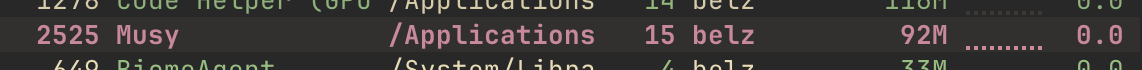
\includegraphics[width=0.8\textwidth]{media/imagemusyram.png}
            \caption{Rendimiento de la aplicación en MacOs}
            \label{fig:ejemplo}
        \end{figure}

\end{document}